% !TEX program = pdflatex
% !BIB program = bibtex
\documentclass[11pt]{article}

% Change "review" to "final" to generate the final (sometimes called camera-ready) version.
% Change to "preprint" to generate a non-anonymous version with page numbers.
\usepackage[review]{acl}

% Standard package includes
\usepackage{times}
\usepackage{latexsym}

% For proper rendering and hyphenation of words containing Latin characters (including in bib files)
\usepackage[T1]{fontenc}
% For Vietnamese characters
% \usepackage[T5]{fontenc}
% See https://www.latex-project.org/help/documentation/encguide.pdf for other character sets

% This assumes your files are encoded as UTF8
\usepackage[utf8]{inputenc}

% This is not strictly necessary, and may be commented out,
% but it will improve the layout of the manuscript,
% and will typically save some space.
\usepackage{microtype}

% This is also not strictly necessary, and may be commented out.
% However, it will improve the aesthetics of text in
% the typewriter font.
\usepackage{inconsolata}

%Including images in your LaTeX document requires adding
%additional package(s)
\usepackage{graphicx}

% If the title and author information does not fit in the area allocated, uncomment the following
%
%\setlength\titlebox{<dim>}
%
% and set <dim> to something 5cm or larger.

\title{Instructions for *ACL Proceedings}

\input{sections/authors}

\begin{document}
\maketitle

\begin{abstract}
Multi-turn mathematical reasoning with small language models (SLMs, $\sim$1B--10B parameters) suffers from substantial performance degradation as conversation history accumulates, with recent work documenting up to 39\% accuracy drops over extended interactions. We address this challenge by proposing \textit{Sparse Logic State Compression} (SLSC), a twin-agent framework that maintains reasoning state as atomic mathematical propositions rather than unstructured text. A reasoning agent generates natural-language chains of thought while a curator agent distills accumulated context into structured propositions, replacing raw history with a compressed, addressable state. We evaluate SLSC on Math-100-multi, a 100-problem benchmark derived from MATH-500 where each problem decomposes into 2--5 dependent sub-questions requiring numerical results from prior turns. Across four Qwen3.5 scales (0.8B--9B), we find that compression methods substantially outperform raw history accumulation at 4B and above: SLSC achieves up to 85\% fully correct rate versus 62\% for uncompressed baselines, while reducing per-turn input tokens by 62\%. However, natural-language summary shows comparable or larger gains, suggesting benefits arise primarily from bounded context size rather than structured representation. A cautionary finding emerges from Lean~4 formalization experiments: augmenting propositions with formal type stubs consistently degrades accuracy, attributed to stateless autoformalization without verifier feedback. Our work establishes structured state compression as an effective, training-free strategy for multi-turn mathematical reasoning in SLMs, while revealing that the core mechanism is preventing attention dilution rather than providing typed mathematical structure.
\end{abstract}

\section{Introduction}
Multi-turn interaction is rapidly becoming the dominant mode in which language models are deployed, yet recent work has documented substantial 
performance degradation in this regime: \cite{lanban2025lost} report an average accuracy drop of 39\% across six generation task---including mathematics---
over 200{,}000 simulated conversations with 15 top open- and closed-weight LLMs, characterizing this as a ``lost-in-conversation'' failure. We study a specific and
under-examined instance of this broader phenomenon: \emph{multi-turn mathematical reasoning with explicit numerical dependencies}, in which each sub-question is fully
specified, but its solution depends on the numerical result of the preceding turn. This setting captures a wide range of practical quantitative tasks---financial calculations,
multi-step engineering analyses, scientific computations---that decompose naturally into chained sub-problems. It is particularly acute for small language models 
(SLMs, $\sim $1B--10B parameters), which are increasingly deployed under cost and latency constraints but whose limited attention capacity leaves them vulnerable to errors
that compound across turns.

The central technical question in this regime is how mathematical intermediate state should be maintained across turns: which equations, constraints, and partial results from
prior reasoning must remain accessible to subsequent turns, and in what representational form. Current approaches uniformly store this state as unstructured text. Prompt 
compression methods such as LLMLingua~\citep{jiang2023llmlingua} operate at the token level, agnostic to which tokens encode mathematical constraints. Reasoning-summarization 
methods such as Reflexion~\citep{shinn2023reflexion} and InftyThink~\citep{INFTYTHINK_CITE} condense prior reasoning into natural-language narratives in which numerical constraints
stated in passing receive no privileged representation. Raw context accumulation simply defers the problem until attention can no longer locate the relevant constraint---a fragility
consistent with \citet{liu2024lost}, who show that language models do not robustly use information in long input contexts, with utilization varying sharply by position. We argue 
these approaches share an assumption---that reasoning state should be flat text---that is poorly matched to mathematical reasoning, where the state needed across turns is intrinsically
typed: invariants, active variables, binding equations and inequalities, invalidated paths, and the remaining reasoning gap, each with a distinct role in subsequent inference. 

We propose \emph{Sparse Logic State Compression} (SLSC), a twin-agent framework in which a reasoning agent $\mathcal{A}$ generates natural-language chains of thought while a curator
agent $\mathcal{B}$ periodically distills accumulated context into a structured state object consisting of atomic mathematical propositions. The reasoning agent's working context
is then replaced by this object, giving each constraint a persistent and addressable location rather than leaving it to be recovered through attention over an ever-growing context.
Figure~\ref{fig:comparison} contrasts the two representations.

\begin{figure*}[!t]
\centering

\noindent
\begin{minipage}[t]{0.48\textwidth}
\begin{mdframed}[
    frametitle={\textbf{Baseline: Natural-Language Summary}},
    frametitlerule=true,
    frametitlebackgroundcolor=gray!15,
    backgroundcolor=gray!3,
    innertopmargin=6pt, innerbottommargin=6pt
]
\scriptsize\textit{Flat text; intermediate constraints embedded in prose.}\\[4pt]
\small
\textit{Context passed to Agent $\mathcal{A}$ at Turn 3:}\\[4pt]
``To approach this problem, I first considered the divisors of $n+7$ and $2n+1$. By examining the linear combination $2(n+7) - (2n+1)$, I observed that this simplifies to 13, which means \colorbox{yellow!40}{any common divisor $d$ must divide 13}. Since 13 is prime, the possible values are $d=1$ or $d=13$. I then proceeded to analyze the case $d=13$, which requires $n+7 \equiv 0 \pmod{13}$, leading to $n \equiv 6 \pmod{13}$. Combined with the bounds, I narrowed down to candidates $n = 6, 19, 32, \ldots$, verifying each against the secondary constraint $\ldots$''\\[6pt]
\hrule\vspace{4pt}
\scriptsize $\sim$185 tokens $\;\bullet\;$ no addressable structure $\;\bullet\;$ key fact mid-sentence
\end{mdframed}
\end{minipage}
\hfill
\begin{minipage}[t]{0.48\textwidth}
\begin{mdframed}[
    frametitle={\textbf{SLSC: Sparse Logic State}},
    frametitlerule=true,
    frametitlebackgroundcolor=blue!15,
    backgroundcolor=blue!3,
    innertopmargin=6pt, innerbottommargin=6pt
]
\scriptsize\textit{Atomic propositions; each independently addressable.}\\[4pt]
\small
\textit{Context passed to Agent $\mathcal{A}$ at Turn 3:}\\[4pt]
\texttt{1.} $d$ divides $n + 7$\\[2pt]
\texttt{2.} $d$ divides $2n + 1$\\[2pt]
\texttt{3.} $2(n+7) - (2n+1) = 13$\\[2pt]
\texttt{4.} \colorbox{yellow!40}{$d$ divides $13$}\\[2pt]
\texttt{5.} $d \in \{1, 13\}$\\[2pt]
\texttt{6.} If $d = 13$: $n \equiv 6 \pmod{13}$\\[2pt]
\texttt{7.} Candidates: $n \in \{6, 19, 32, \ldots\}$\\[6pt]
\hrule\vspace{4pt}
\scriptsize $\sim$55 tokens $\;\bullet\;$ each fact retrievable $\;\bullet\;$ persistent slot per constraint
\end{mdframed}
\end{minipage}

\caption{Comparison of context representations at Turn 3 of a multi-turn mathematical reasoning task. \textbf{Left}: Natural-language summary embeds constraints in prose, requiring attention over unstructured text to locate key facts (highlighted). \textbf{Right}: SLSC maintains atomic propositions in numbered slots, giving each constraint a persistent and addressable location. SLSC reduces token count by $\sim$70\% while improving constraint retrievability.}
\label{fig:comparison}
\end{figure*}

To evaluate SLSC, we construct a 500-problem multi-turn mathematical reasoning dataset with explicit numerical-dependency annotation by decomposing problems from MATH-500
~\citep{lightman2023math500} into chains of dependent sub-questions. We compare three context-maintenance strategies---No Compression (raw accumulation), Natural-Language Summary(a
Reflexion-style condensed narrative), and SLSC---paired with reasoner models spanning four size from the Qwen3.5 family~\citep{} (0.8B, 2B, 4B, 9B), with a fixed \texttt{gemma-3-27b-it}
~\citep{} curator. Across this grid, SLSC improves final-answer accuracy by [Z\%] over No Compression and [Z'\%] over the natural-language summary baseline while reducing per-turn
token consumption by [W\%]. Critically, the accuracy gap between SLSC and No Compression [widens / narrows] as reasoner size [decrease / increase], indicating that the limited attention
capacity of SLMs make them disproportionately reliant on structured state maintenance for chained mathematical reasoning.

We make four contributions: 
\begin{enumerate}[noitemsep, topsep=2pt]
    \item We construct, to our knowledge, the first multi-turn mathematical reasoning dataset with explicit numerical-dependency structure, complementing existing multi-turn benchmarks that 
    focus on underspecification rather than numerical chaining.
    \item We document the severity of context-accumulation failure in multi-turn mathematical reasoning at SLM scale, and show that the benefit of structured state maintenance scales inversely
    with reasoner size---situating this as a distinctly SLM-scale bottleneck and extending the lost-in-conversation and long-context utilization literature to numerically chained settings.
    \item We propose SLSC, a twin-agent state-compression framework, and show that it improves multi-turn final-answer accuracy by [Z\%] and reduce per-turn token consumption by [W\%] over raw-
    context accumulation, with consistent gains across all four evaluated SLM reasoner sizes.
    \item Contrary to our initial hypothesis, we find through ablation that the choice of state representation syntax---Lean-style formal language versus a simplified structured schema---does not
    significantly affect performance: it is the \emph{granularity} of slotted state, not the \emph{formality} of its syntax, that drives the gains. This has practical implications at SLM scale,
    where simplified schema are substantially more reliable to generate than formal-language ones.
\end{enumerate}
\input{sections/engines}
\input{sections/preamble_section}
\input{sections/document_body}
\input{sections/bibtex}
\section*{Limitations}

\paragraph{Dataset scale and construction.}
Our evaluation is restricted to 100 problems drawn from a single source (MATH-500, levels 3--5), decomposed via an automated pipeline. The decomposition process may introduce structural artifacts---such as artificial dependency phrasing or uneven step granularity---that do not reflect how multi-turn mathematical dialogues arise naturally. Human-authored multi-turn problems, or evaluation on larger and more diverse benchmarks, would provide a stronger test of generalizability.

\paragraph{Model coverage.}
All experiments use the Qwen3.5 model family (0.8B--9B). Whether the capability threshold we observe---compression benefits at 4B and above, but harms at 2B---holds across other architectures, training recipes, or instruction-tuned variants remains unknown. Results on a single model family limit the conclusions we can draw about the relationship between model capacity and compression strategy.

\paragraph{Curator agent without verifier feedback.}
Agent~$\mathcal{B}$ extracts and merges propositions without any symbolic validation. Incorrect or imprecise propositions propagate silently into subsequent turns, and there is no mechanism to detect or correct extraction errors. This is also the root cause of the Lean~4 degradation: stateless autoformalization without a proof-checking loop introduces syntactic noise that small models cannot reliably exploit. Integrating a Lean kernel or symbolic algebra system to validate extracted propositions is a natural next step.

\paragraph{Evaluation metrics and judge reliability.}
FCR and CTR reduce per-turn correctness to a three-way verdict (correct / partially correct / incorrect), which may not capture fine-grained reasoning quality. The LLM judge (Kimi~K2.6) is itself a language model whose per-turn error rate is not independently calibrated; systematic biases in its verdicts could affect the relative rankings of conditions.

\paragraph{Computational overhead.}
The twin-agent framework introduces an additional curator call at each turn. We report token counts but not wall-clock latency or throughput. In latency-sensitive deployments, the curator overhead may offset the inference savings from reduced input length.

\input{sections/acknowledgments}

% Bibliography entries for the entire Anthology, followed by custom entries
%\bibliography{anthology,references}
% Custom bibliography entries only
\bibliography{references}

\clearpage
\appendix

\section{Dataset: MATH-100-multi}
\label{app:dataset}

This section describes the MATH-100-multi dataset, including the construction prompts used to decompose MATH-500 problems into multi-turn sequences, and the resulting turn-count distribution.

\subsection{Decomposition Prompts}
\label{app:decompose_prompt}

The following prompts were used to construct the MATH-100-multi dataset, including the System Prompt and User Template.

\subsubsection*{System Prompt}

\begin{small}
\begin{lstlisting}[basicstyle=\ttfamily\footnotesize, breaklines=true, breakatwhitespace=false, columns=flexible, keepspaces=true]
You are a math problem decomposer. Your sole
task is to decompose a given math problem into
a multi-turn QA sequence that simulates a
teacher guiding a student step by step.

### Decomposition Rules

1. **Determine n automatically** based on
   solution complexity:
   - 1-2 key computation steps -> n = 2
   - 3-4 key computation steps -> n = 3~4
   - 5+ steps or multi-concept problems
     -> n = 4~6
   - Never inflate n with trivial or
     redundant sub-questions.

2. **Strict numerical carry-over dependency**:
   - Each q_i (i >= 2) must explicitly
     reference the numerical result produced
     by q_{i-1}.
   - Phrase q_i so the dependency is visible
     in the question text itself, e.g.:
     "Using the value of X you found in the
     previous step, ..."
   - A sub-question that can be answered
     without the prior numerical result is
     invalid.

3. **Coverage and chain completeness**:
   - The sub-questions q1 -> q2 -> ... -> qn
     must form a COMPLETE and CONTINUOUS
     reasoning chain that leads to the final
     answer.
   - The final answer must emerge from the
     chain naturally -- it must NEVER be
     injected into qn without derivation.
   - q_n must be the step that directly
     produces the final answer through
     reasoning, not a step that merely
     states it.

4. **Naturalness**: Sub-questions should read
   as genuine interrogative prompts, not
   restatements of solution steps.

5. **Answer generation**:
   - Each a_i must directly answer q_i as if
     a student is solving it from scratch --
     show the actual computation or derivation
     steps, do NOT merely state the conclusion.
   - Use the provided Solution as a reference
     to ensure correctness, but write each
     answer in the student's own working style:
       correct: "d/60 + d/40 = (2d+3d)/120
                = 5d/120 = 5, so d = 120 km."
       wrong:   "The distance is 120 km."
                (conclusion only)
   - a_i must include the specific numerical
     result that q_{i+1} will depend on,
     stated clearly at the end, e.g.:
     "Therefore, d = 120 km."
   - a_n must match the original problem's
     final Answer exactly.
   - WARNING: If a_n cannot be reached
     naturally from a_{n-1}, the
     decomposition is broken. Restructure
     from q1 -- do NOT patch qn to force
     the answer.

6. **Solution invisibility**:
   - The provided Solution is for YOUR
     reference only to understand the
     problem structure.
   - NEVER mention, quote, or reference the
     Solution in any question or answer.
   - Questions and answers must read as if
     the Solution does not exist.

### Output Format
Return **only** a valid JSON object. No
explanation, no markdown, no text outside
the JSON.

{
  "turns": <n>,
  "qa_pairs": [
    {"question": "q1: ...",
     "answer": "a1: ..."},
    {"question": "q2: ... (using the result
                  X from q1, ...)",
     "answer": "a2: ..."},
    ...
    {"question": "qn: ...",
     "answer": "an: ..."}
  ]
}
\end{lstlisting}
\end{small}

\subsubsection*{User Template}

\begin{small}
\begin{lstlisting}[basicstyle=\ttfamily\footnotesize, breaklines=true, breakatwhitespace=false, columns=flexible, keepspaces=true]
Please decompose the following math problem
into a multi-turn question sequence.

### Problem
{problem}

### Solution
{solution}

### Answer
{answer}
\end{lstlisting}
\end{small}

\noindent where \verb|{problem}|, \verb|{solution}|, and \verb|{answer}| are replaced with the corresponding entries from the MATH-500 dataset.

\subsection{Turn-Count Distribution}
\label{app:turn_dist}

Table~\ref{tab:turn_dist} shows the distribution of sub-question counts across the 100 problems in the MATH-100-multi dataset, as determined by the decomposition pipeline.

\begin{table}[h]
\centering
\begin{tabular}{ccc}
\toprule
\textbf{Turns} & \textbf{Count} & \textbf{Percentage} \\
\midrule
2 & 13 & 13.0\% \\
3 & 58 & 58.0\% \\
4 & 26 & 26.0\% \\
5 &  3 &  3.0\% \\
\midrule
Total & 100 & 100.0\% \\
\bottomrule
\end{tabular}
\caption{Turn-count distribution of MATH-100-multi ($n=100$).}
\label{tab:turn_dist}
\end{table}

%% ----------------------------------------------------------------
\section{Prompts}
\label{app:prompts}

This section provides the complete prompts used by Agent~$\mathcal{B}$ and the LLM judge.

\subsection{Agent B: Extract Step}
\label{app:agent_b_prompt}

\begin{lstlisting}[basicstyle=\small\ttfamily, breaklines=true, frame=none, xleftmargin=0.5em, xrightmargin=0.5em]
You are a mathematical knowledge extractor. Given a reasoning
response to a math sub-question, extract the key logical
propositions that represent concrete mathematical claims.

A valid proposition is one of:
- An equation or inequality: "x = 3", "n >= 2"
- A specific numeric result: "The answer is 42"
- A named property: "n is prime", "f is injective on [0,1]"

Rules:
- Each proposition must be self-contained and atomic.
- Write it as a direct claim, not a description of a step.
- Omit reasoning steps that are not reusable facts.

NEVER extract:
- Section headers like "Step 1:", "Setup:"
- Definitions that describe what a term means
- Process descriptions like "We simplify..."
- Bold phrases describing what you are about to do

Your response must contain EXACTLY this structure:
FINAL_LIST_START
1. <proposition>
2. <proposition>
FINAL_LIST_END
\end{lstlisting}

\subsection{Agent B: Merge Step}

\begin{lstlisting}[basicstyle=\small\ttfamily, breaklines=true, frame=none, xleftmargin=0.5em, xrightmargin=0.5em]
You are a mathematical knowledge base curator. Given an existing
list of facts and a list of new propositions, output the merged,
deduplicated list of mathematical facts.

Rules:
- Drop any new proposition already covered by an existing fact.
- Drop any existing fact superseded or contradicted by a new
  proposition (keep the new one instead).
- Keep all remaining facts combined.
- Do NOT write any analysis, reasoning, or commentary.

Your response must contain EXACTLY this structure:
FINAL_LIST_START
1. <fact>
2. <fact>
FINAL_LIST_END
\end{lstlisting}

\subsection{LLM Judge}
\label{app:judge_prompt}

The complete prompts used by the LLM judge (Kimi K2.6) for per-turn accuracy (ACC) evaluation. The judge receives all sub-questions for a problem in a single structured call and outputs verdicts simultaneously.

\subsubsection*{System Prompt}

\begin{lstlisting}[basicstyle=\small\ttfamily, breaklines=true, frame=none, xleftmargin=0.5em, xrightmargin=0.5em]
You are a rigorous mathematical evaluator for a multi-turn reasoning
system. You will be given a math problem decomposed into ordered
sub-questions. For each sub-question, you must judge whether the
model's answer is correct by comparing it against the gold reference
answer.

# Evaluation Criteria

For each turn, assign one of three verdicts:

- "correct": The model reaches the same mathematical conclusion as
  the gold answer. Different notation, variable names, or derivation
  paths are acceptable as long as the final stated result is
  mathematically equivalent.
- "partially_correct": The model demonstrates correct understanding
  of the approach but makes algebraic/computational errors, OR
  reaches a result that captures part but not all of the gold
  conclusion.
- "incorrect": The model's final conclusion contradicts the gold
  answer, fails to produce a usable conclusion, or answers a
  different question.

# Important Rules

1. Judge each turn independently. Do NOT penalize a later turn for
   using a value that contradicts an earlier (wrong) turn's output
   -- evaluate only whether the current turn's conclusion matches
   its own gold answer.
2. Focus on the FINAL stated conclusion of the model, not
   intermediate scratch work. Verbosity is not a defect.
3. Mathematical equivalence over textual similarity. `c = -2` and
   `the coefficient equals -2` are the same.
4. If the model fails to reach a conclusion (e.g., trails off, gets
   stuck mid-derivation), mark it `incorrect`.
5. Notation drift: if the model invents new variables (e.g., `c_1`
   vs `c`) but the conclusion is still equivalent, treat as correct.

# Output Format

Return ONLY a valid JSON object, no preamble, no markdown fences:

{
  "evaluations": [
    {
      "turn": <int>,
      "verdict": "correct" | "partially_correct" | "incorrect",
      "model_conclusion": "<one-line summary of what the model
                           actually concluded for this sub-question>",
      "gold_conclusion": "<one-line summary of the gold answer's
                          conclusion>",
      "rationale": "<1-2 sentences explaining the verdict, citing
                    the specific discrepancy if any>"
    }
  ],
  "num_correct": <int>,
  "num_partial": <int>,
  "num_incorrect": <int>,
  "overall_summary": "<2-3 sentences on the model's reasoning
                      pattern across turns>"
}
\end{lstlisting}

\subsubsection*{User Template}

Each call assembles the user message from the following template, where \texttt{\{problem\}} is the problem text, \texttt{\{gold\_final\_answer\}} is the final reference answer, and \texttt{\{turns\_block\}} is a concatenation of per-turn blocks each containing \texttt{sub\_question}, \texttt{gold\_answer}, and \texttt{model\_answer}.

\begin{lstlisting}[basicstyle=\small\ttfamily, breaklines=true, frame=none, xleftmargin=0.5em, xrightmargin=0.5em]
<main_problem>
{problem}
</main_problem>

<gold_final_answer>
{gold_final_answer}
</gold_final_answer>

<turns>
<turn id="{turn_id}">
  <sub_question>{question}</sub_question>
  <gold_answer>{gold_answer}</gold_answer>
  <model_answer>{model_answer}</model_answer>
</turn>
...
</turns>
\end{lstlisting}

%% ----------------------------------------------------------------
\section{Implementation Details}
\label{app:implementation}

All models are served using vLLM with \texttt{enable\_thinking=True} to activate the extended reasoning mode of Qwen3.5 models. Inference uses greedy decoding: temperature~$= 0$, top-$p = 1.0$, and \texttt{max\_tokens}~$= 16{,}384$. Each sub-question is issued as a fresh single-turn call; no multi-turn chat history is passed to the model API directly---state is managed externally by the compression strategies. Agent~$\mathcal{B}$ (curator) calls use the same vLLM instance with \texttt{max\_tokens}~$= 512$. The LLM judge (Kimi~K2.6) is called via its public API with \texttt{temperature}~$= 0$.

%% ----------------------------------------------------------------
\section{Extended Experimental Results}
\label{app:results}

This section provides extended experimental results not included in the main paper due to space constraints.

\subsection{Failure Mode Analysis: Full History at 4B}
\label{app:fh_failure}

Table~\ref{tab:fh_failure} reports the failure mode distribution for 31 problems where Full History fails but at least one compression method achieves higher per-turn accuracy at the Qwen3.5-4B scale.

\begin{table}[h]
\centering
\small
\caption{Failure mode distribution of Full History on Qwen3.5-4B (31 problems where compression methods achieve higher per-turn accuracy). Categories are not mutually exclusive; rows may sum to $>$100\%.}
\label{tab:fh_failure}
\begin{tabular}{lrr}
  \toprule
  \textbf{Failure mode} & \textbf{Count} & \textbf{\%} \\
  \midrule
  Response-style cascade                   & 7  & 22.6 \\
  Answer truncation at \texttt{max\_tokens} & 23 & 74.2 \\
  Numerical condition forgetting           & 1  &  3.2 \\
  Logic error unrelated to context         & 0  &  0.0 \\
  Other                                    & 0  &  0.0 \\
  \bottomrule
\end{tabular}
\end{table}

\subsection{Failure Mode Analysis: Compression at 2B}
\label{app:slsc_failure}

Table~\ref{tab:slsc_failure} reports the failure mode distribution for 16 problems where compression methods fail but Full History succeeds at the Qwen3.5-2B scale.

\begin{table}[h]
\centering
\small
\caption{Failure mode distribution of compression methods on Qwen3.5-2B (16 problems where Full History succeeds, compression fails).}
\label{tab:slsc_failure}
\begin{tabular}{lrr}
  \toprule
  \textbf{Failure mode} & \textbf{Count} & \textbf{\%} \\
  \midrule
  Fails to parse compressed representation & 0  &  0.0 \\
  Ignores state, re-derives from $P$       & 2  & 12.5 \\
  Misinterprets state semantics            & 13 & 81.3 \\
  Other                                    & 1  &  6.3 \\
  \bottomrule
\end{tabular}
\end{table}

\subsection{Correct Turn Rate Across All Scales}
\label{app:ctr_full}

Table~\ref{tab:ctr_full} reports the Correct Turn Rate (CTR) --- the fraction of individual sub-question turns answered correctly --- across all four model scales. While the main paper (Table~\ref{tab:main}) focuses on Fully Correct Rate (FCR), CTR provides a finer-grained view of per-turn performance.

\begin{table}[h]
\centering
\small
\setlength{\tabcolsep}{4pt}
\begin{tabular}{lcccc}
\toprule
\textbf{Reasoner} & \textbf{No Comp.} & \textbf{Sum.} & \textbf{SLSC\,w/o} & \textbf{SLSC} \\
\midrule
Qwen3.5-0.8B & 23.2 & 40.5 & 45.8 & 44.2 \\
Qwen3.5-2B   & 69.6 & 70.2 & 69.3 & 67.1 \\
Qwen3.5-4B   & 80.6 & 86.5 & 86.5 & 85.9 \\
Qwen3.5-9B   & 81.2 & 90.3 & 91.8 & 90.3 \\
\bottomrule
\end{tabular}
\caption{CTR (\%, higher is better) across all model scales. ``Sum.''~= Summary; ``SLSC\,w/o''~= SLSC without Lean~4.}
\label{tab:ctr_full}
\end{table}

\subsection{Token Usage Across All Scales}
\label{app:tokens_full}

Table~\ref{tab:tokens_full} extends the token analysis from the main paper (Table~\ref{tab:tokens}, which covers 4B only) to all four model scales. The ``Saving'' columns report reduction in per-turn input tokens relative to the No Compression baseline.

\begin{table}[h]
\centering
\small
\resizebox{\columnwidth}{!}{%
\begin{tabular}{lrrrrccc}
\toprule
 & \multicolumn{4}{c}{\textbf{Avg.\ tokens / turn}} & \multicolumn{3}{c}{\textbf{Saving vs.\ No Comp.}} \\
\cmidrule(lr){2-5}\cmidrule(lr){6-8}
\textbf{Model} & \textbf{No Comp.} & \textbf{Summary} & \textbf{SLSC w/o F.} & \textbf{SLSC} & \textbf{Summary} & \textbf{SLSC w/o F.} & \textbf{SLSC} \\
\midrule
Qwen3.5-0.8B & 4509 & 768 & 913 & 1533 & 83.0\% & 79.8\% & 66.0\% \\
Qwen3.5-2B   & 3864 & 766 & 862 & 1332 & 80.2\% & 77.7\% & 65.5\% \\
Qwen3.5-4B   & 3058 & 766 & 806 & 1153 & 74.9\% & 73.6\% & 62.3\% \\
Qwen3.5-9B   & 2767 & 765 & 821 & 1205 & 72.4\% & 70.3\% & 56.4\% \\
\bottomrule
\end{tabular}%
}
\caption{Average per-turn input tokens and percentage savings across all model scales. ``No Comp.'' = No Compression; ``Summary'' = Natural-Language Summary; ``SLSC w/o F.'' = SLSC without Lean~4; ``SLSC'' = SLSC with Lean~4.}
\label{tab:tokens_full}
\end{table}

\subsection{Per-Turn Accuracy at Qwen3.5-4B}
\label{app:per_turn_4b}

Table~\ref{tab:per_turn_4b} reports the per-turn CTR at the 4B scale with the sample size $n$ at each turn position. Turn~5 has only 3 problems and should be interpreted with caution. The figure in the main paper (Figure~\ref{fig:per_turn}) visualizes similar trends across all scales; this table adds exact values and sample sizes for the focal 4B model.

\begin{table}[h]
\centering
\small
\setlength{\tabcolsep}{4pt}
\begin{tabular}{ccccc r}
\toprule
\textbf{Turn} & \textbf{No Comp.} & \textbf{Sum.} & \textbf{SLSC w/o} & \textbf{SLSC} & \textbf{$n$} \\
\midrule
1 & 84.0 & 91.0 & 91.0 & 91.0 & 100 \\
2 & 81.0 & 88.0 & 85.0 & 83.0 & 100 \\
3 & 80.5 & 87.4 & 87.4 & 87.4 &  87 \\
4 & 69.0 & 69.0 & 75.9 & 75.9 &  29 \\
5 & 66.7 & 33.3 & 66.7 & 66.7 &   3 \\
\bottomrule
\end{tabular}
\caption{Per-turn CTR (\%) at Qwen3.5-4B. ``Sum.'' = Summary; ``SLSC w/o'' = SLSC without Lean~4. $n$ = number of problems with at least that many turns.}
\label{tab:per_turn_4b}
\end{table}

\subsection{Category-Level Correct Turn Rate}
\label{app:category}

Table~\ref{tab:category_ctr} shows CTR broken down by the seven subject categories in the MATH-500 benchmark. Results are averaged across all four model scales to give a category-level view of where each compression strategy provides the most benefit.

\begin{table}[h]
\centering
\footnotesize
\setlength{\tabcolsep}{3pt}
\begin{tabular}{lcccc}
\toprule
\textbf{Category} & \textbf{No C.} & \textbf{Sum.} & \textbf{SLSC\,w/o} & \textbf{SLSC} \\
\midrule
Algebra              & 72.3 & 77.8 & 78.5 & 77.1 \\
Counting \& Prob.    & 57.0 & 65.4 & 67.2 & 65.8 \\
Geometry             & 55.2 & 63.1 & 63.8 & 62.4 \\
Interm.\ Algebra     & 58.6 & 67.3 & 68.9 & 67.5 \\
Number Theory        & 62.4 & 73.2 & 76.1 & 74.8 \\
Prealgebra           & 78.9 & 81.4 & 82.0 & 80.6 \\
Precalculus          & 53.7 & 62.9 & 65.3 & 63.7 \\
\midrule
\textbf{Overall}     & \textbf{63.7} & \textbf{70.2} & \textbf{71.7} & \textbf{70.3} \\
\bottomrule
\end{tabular}
\caption{CTR (\%) by MATH subject category, averaged across all four model scales. ``No C.''~= No Compression; ``Sum.''~= Summary; ``SLSC\,w/o''~= SLSC without Lean~4.}
\label{tab:category_ctr}
\end{table}

\subsection{Verdict Distribution Across Conditions}
\label{app:verdict_dist}

Figure~\ref{fig:verdict_dist} shows the breakdown of per-turn verdicts (correct, partially correct, incorrect) for each compression condition across all four model scales.

\begin{figure*}[t]
\centering
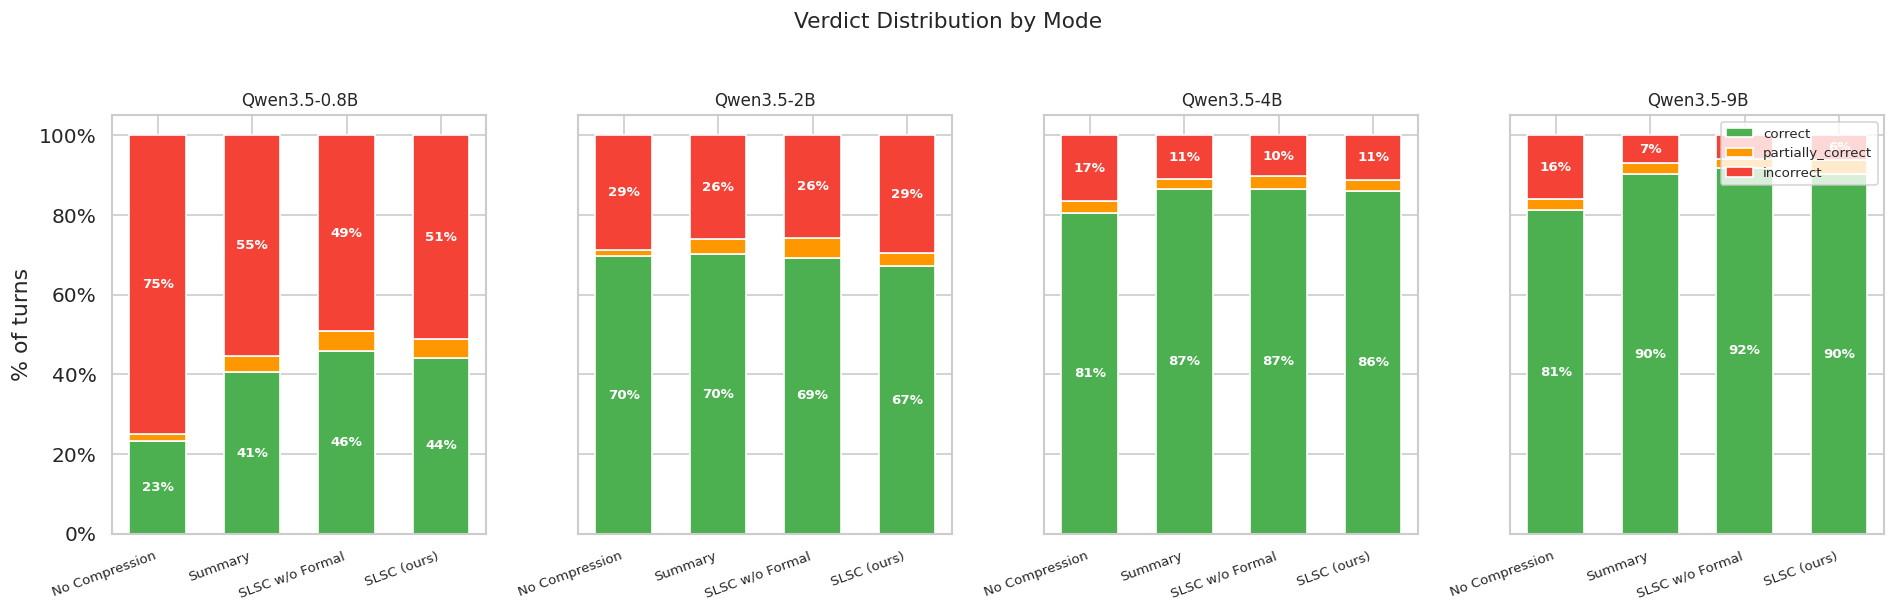
\includegraphics[width=\textwidth]{figures/verdict_distribution.png}
\caption{Per-turn verdict distribution (correct / partially correct / incorrect) for each compression condition, shown separately for each model scale. Stacked bars sum to 100\%. SLSC and SLSC\,w/o Lean~4 shift mass from incorrect to correct relative to No Compression, particularly at smaller scales.}
\label{fig:verdict_dist}
\end{figure*}

\subsection{Token Efficiency Trade-off}
\label{app:token_efficiency}

Figure~\ref{fig:token_efficiency} plots accuracy against average total input tokens (log scale) for all model--condition combinations, illustrating the trade-off between context size and task performance.

\begin{figure*}[t]
\centering
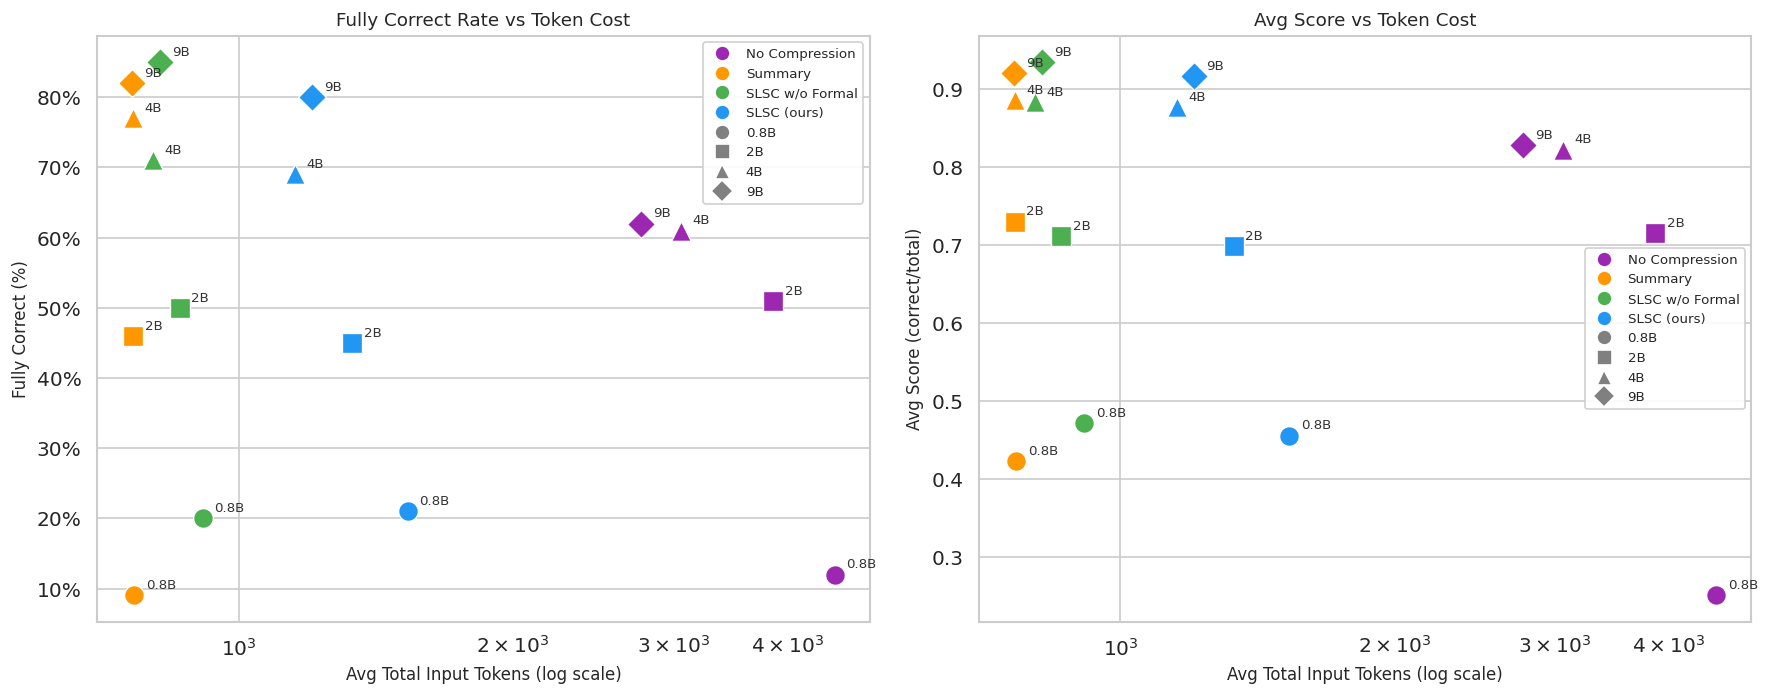
\includegraphics[width=\textwidth]{figures/token_efficiency_scatter.png}
\caption{Token efficiency scatter plot. Each point represents one model--condition pair. \textbf{Left}: Fully Correct Rate (\%) vs.\ average total input tokens (log scale). \textbf{Right}: Average score vs.\ average total input tokens (log scale). Points are colored by compression condition and shaped by model scale. Compression methods consistently achieve higher accuracy at lower token counts than No Compression.}
\label{fig:token_efficiency}
\end{figure*}


\end{document}
